% Fig 2.12 / spec Fig A07 -- a single point carries no area, hence no
% probability.  Source: mathstatch2.tex lines 761-796.
% Per spec 1.6 the schematic curve 2 e^{-(t-3)^2/2} is replaced by the true
% N(3,1) density f(t) = 0.3989423 e^{-(t-3)^2/2}, which integrates to 1.
% Drawing scale x=1.15cm, y=8.74cm; peak f(3) = 0.3989423 -> 3.4868cm.
% The shaded region of Figs 2.8 and 2.11 has here collapsed onto the single
% segment at a = 3.5, drawn in the accent colour: it has no width, so no area.
\documentclass[tikz,border=2pt]{standalone}
\usepackage{amsmath}
\usepackage{amssymb}
\usepackage{xcolor}
\usetikzlibrary{arrows.meta}
\newcommand{\sssig}{\scriptscriptstyle}

\definecolor{journalink}{HTML}{1F1C18}
\definecolor{journalmuted}{HTML}{8A7F72}
\definecolor{journalaccent}{HTML}{9C2D2D}

\begin{document}
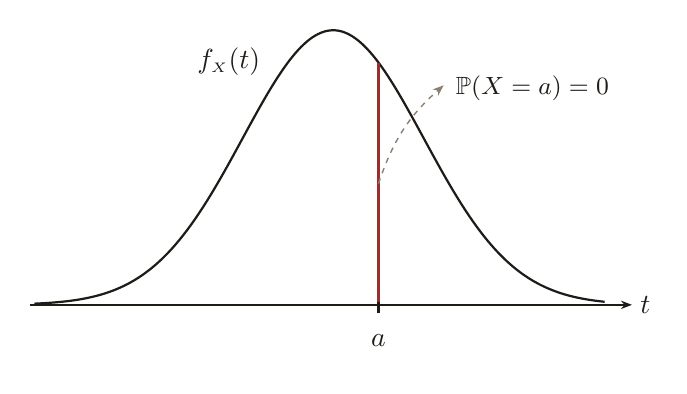
\begin{tikzpicture}[
  x=1.15cm,
  y=8.74cm,
  every node/.style={font=\normalsize, journalink},
  axis/.style={journalink, line width=0.8pt, -{Stealth[length=4pt]}},
  tick/.style={journalink, line width=0.8pt},
  curve/.style={journalink, line width=0.8pt},
  guide/.style={journalmuted, line width=0.5pt, dash pattern=on 2pt off 2pt},
  degenerate/.style={journalaccent, line width=0.8pt},
  pointer/.style={journalmuted, line width=0.5pt,
                  dash pattern=on 2pt off 2pt, -{Stealth[length=4pt]}}
]
  % ---- common bounding box, identical in all four figures of this group ----
  \path (-0.43cm,-0.78cm) rectangle (7.58cm,3.52cm);

  % ---- x axis ----
  \draw[axis] (-0.35,0) -- (6.3,0);

  % ---- density curve: N(3,1) ----
  \draw[curve] plot[domain=-0.3:6, samples=200, smooth]
    (\x,{0.3989423*exp(-(\x-3)*(\x-3)/2)});

  % ---- the region [a, a]: a segment of zero width at a = 3.5 ----
  \draw[degenerate] (3.5,0) -- (3.5,0.3520653);
  \draw[tick] ([yshift=0.035cm]3.5,0) -- ([yshift=-0.106cm]3.5,0);
  \node[anchor=north] at ([yshift=-0.25cm]3.5,0) {$a$};

  % ---- callout: starts at the midpoint of the degenerate segment and curves
  % up to the label.  The segment runs from (3.5, 0) to (3.5, 0.3520653), so its
  % midpoint is (3.5, 0.17603265); the manuscript does the same, placing the
  % tail at \node (1) at ({\y},{\fy/2}) and bending left (line 772).
  % (2026-08-09, author's ruling.  Two earlier versions are superseded: a
  % straight (3.68,0.360389) -- (4.19,0.314645), whose ends were given different
  % heights so it came out sloping and whose tail sat in blank space above the
  % curve; and (3.56,0.3495) to[bend right=15], which started at the top of the
  % segment instead of its midpoint.  Bend left is used rather than bend right
  % so the arc pulls away from the density curve instead of running alongside
  % it.  The head and the label are unmoved, so the bounding box is unchanged.)
  \draw[pointer] (3.5,0.17603265) to[bend left=15] (4.22,0.3190);
  \node[anchor=east, inner sep=0pt] at ([yshift=2.75cm]6.05,0)
    {\small $\mathbb{P}(X=a)=0$};

  % ---- labels ----
  \node[anchor=south east, inner sep=0pt] at ([yshift=0.38cm]2.2,0.2896916)
    {$f_{\sssig X}(t)$};
  \node[anchor=west, inner sep=2.8pt] at (6.3,0) {$t$};
\end{tikzpicture}
\end{document}
